\documentclass[12pt,a4paper]{report}
\usepackage[utf8]{inputenc}
\usepackage{amsmath}
\usepackage{amsfonts}
\usepackage{amssymb}
\usepackage{graphicx}
\usepackage{lmodern}
\author{Kyle Swanson}
\title{Chapter 6 Exercises: Architecture}

\setlength{\parindent}{0cm}

\begin{document}
\maketitle
\begin{normalsize}

\textbf{Exercise 6.4} - Repeat Exercise 6.3 for memory storage of a 32-bit word stored at memory word 15 in a byte-addressable memory. \\
a) What is the byte address of memory word 15? \\
$ 15 \times 4 = 15 \times 2^{2} = 1111 << 2 $ \\
$ = 111100 = 0x3C $ \\

b) What are the byte address that memory word 15 spans? \\
$ 0x3C to 111100 + 11 $ \\
$ = 111111 = 0x3F $ \\
$ 0x3C to 0x3F $ \\

c) Draw the number 0xFF223344 stored at word 15 in both big-endian and little-endian machines. Your drawing should be similar to Figure 6.4. Clearly label the byte address corresponding to each data byte value. \\
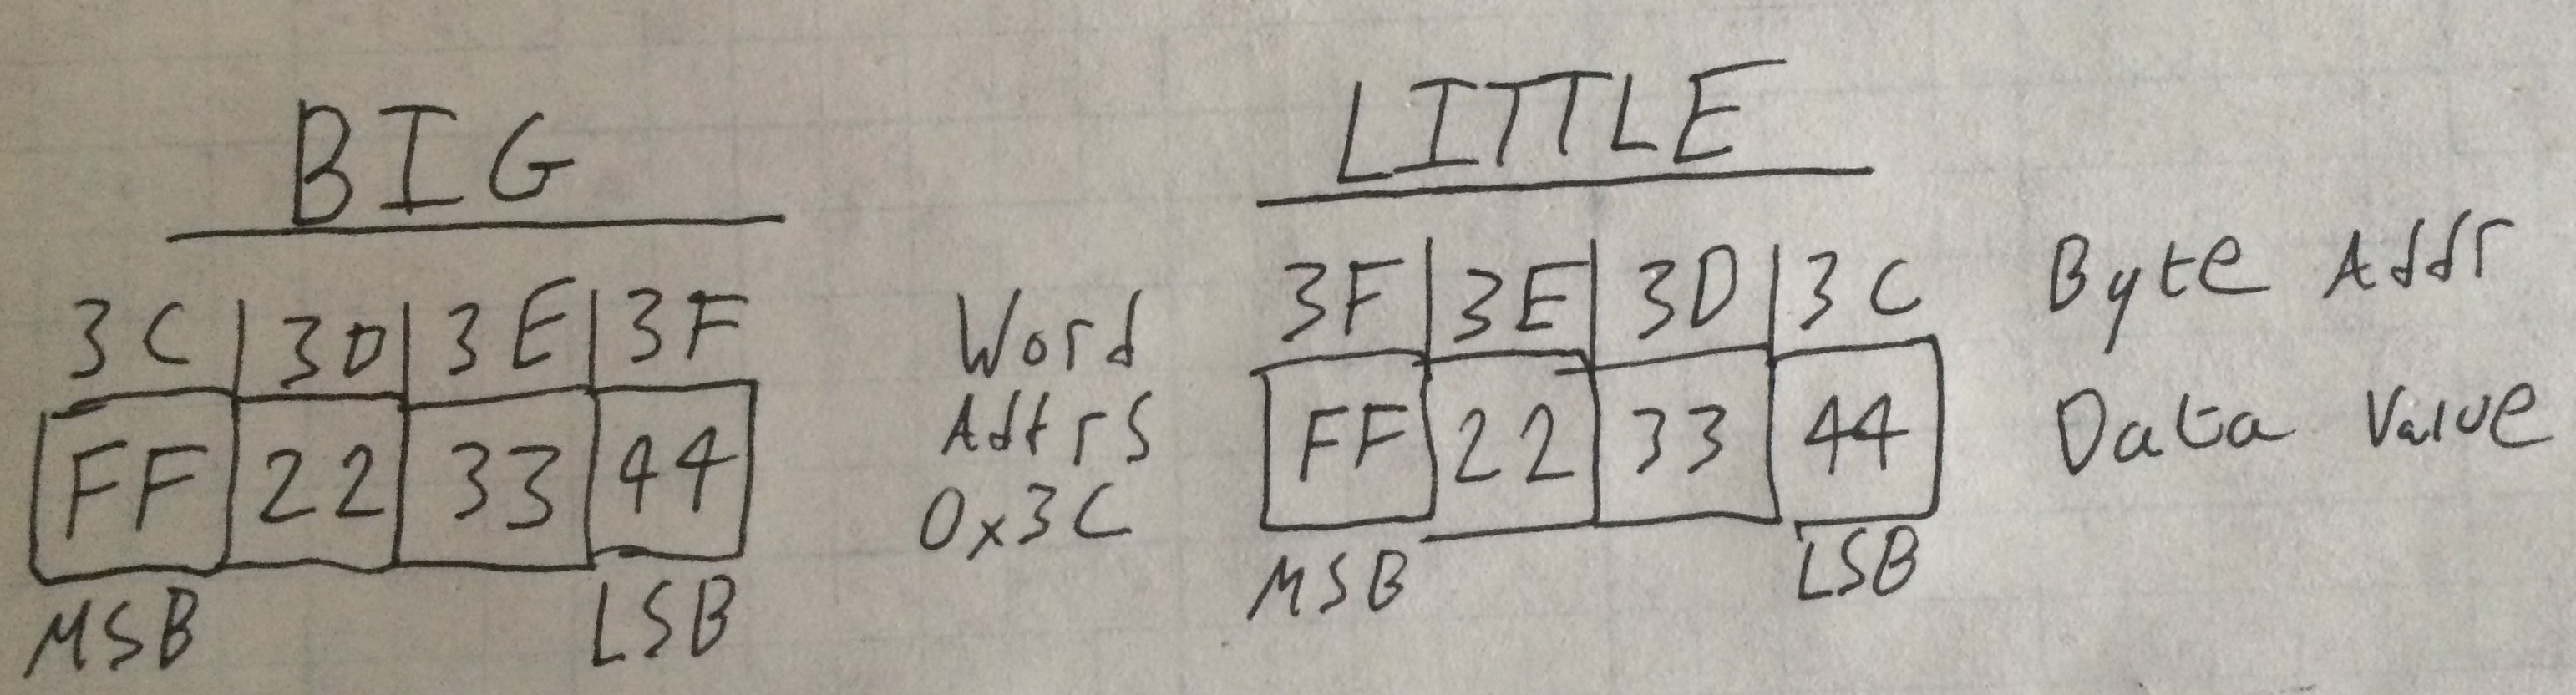
\includegraphics[scale=.15]{img/num} \\


\medskip

\textbf{Exercise 6.10} - Convert the following MIPS assembly code into machine language. Write the instructions in hexadecimal. \\
\textit{add \$t0, \$s0, \$s1} \\
This is an R-type instruction. Add \\
opcode = 000000 \\
rs = \$s0 = 16 = 10000 \\
rt = \$s1 = 17 = 10001 \\
rd = \$t0 = 8 = 01000 \\
shamt = 00000 \\
func = add = 100000 \\

Put it together: \\
000000 10000 10001 01000 00000 100000 \\
= \textbf{0x2114020} \\

\textit{lw \$t0, 0x20(\$t7)} \\
This is a I-type instruction. Load Word - lw rt, imm(rs) \\

opcode = 100011 \\
rs = \$t7 = 15 = 01111 \\
rt = \$t0 = 8 = 01000 \\
imm = 0x20 = 0000000000100000 \\

Put it together: \\
100011 01111 01000 0000000000100000 \\
= \textbf{0x8DE80020} \\

\textit{addi \$s0, \$0, -10} \\
This is a I-type instruction. Add Immediate - addi rt, rs, imm \\

opcode = 001000 \\
rs = 00000 \\
rt = 16 = 10000 \\
imm = -10 = 1111111111110110 \\

Put it together: \\
001000 00000 10000 1111111111110110 \\
= \textbf{0x2010FFF6} \\

\medskip

\textbf{Exercise 6.12} - Consider I-type instructions. \\
a) Which instructions from Exercise 6.10 are I-type instructions? \\
addi and lw are both I-type. \\

b) Sign-extend the 16-bit immediate of each instruction from part (a) so that it becomes a 32bit number. \\
lw immediate = 0000000000100000 \\
Sign extended = 0000000000000000 0000000000100000 = 0x20

addi immediate = 1111111111110110 \\
Sign extended = 1111111111111111 1111111111110110 = 0xFFFFFFF6



\medskip

\textbf{Exercise 6.14 - Do not complete the reverse engineering. Do not explain function. Just convert.} \\

0x20080000 = 001000 00000 01000 0000000000000000 \\
I-type \\
opcode = 001000 = addi \\
rs = 00000 = \$0 \\
rt = 01000 = \$t0 \\
imm = 0000000000000000 = 0 \\

addi \$t0, \$0, 0 \\

0x20090001 = 001000 00000 01001 0000000000000001 \\
I-type \\
opcode = 001000 = addi \\
rs = 00000 = \$0 \\
rt = 01001 = 9 = \$t1 \\
imm = 0000000000000001 = 1\\

addi \$t1, \$0, 1 \\ 

0x0089502A = 000000 00100 01001 01010 00000 101010 \\
R-type \\
opcode = 000000 \\
rs = 00100 = 4 = \$a0 \\
rt = 01001 = 9 = \$t1 \\
rd = 01010 = 10 = \$t2 \\
shamt = 00000 = 0 \\
func = 101010 = slt \\

slt \$t2, \$a0, \$t1 \\

0x15400003 = 000101 01010 00000 0000000000000011 \\
I-type \\
opcode = 000101 = bne \\
rs = 01010 = 10 = \$t2 \\
rt = 00000 = \$0 \\
imm = 0000000000000011 = 3 = 0x3 \\

bne \$t2, \$0, 0x3 \\

0x01094020 = 000000 01000 01001 01000 00000 100000 \\
R-type \\
opcode = 000000 \\
rs = 01000 = 8 = \$t0 \\
rt = 01001 = 9 = \$t1 \\
rd = 01000 = 8 = \$t0 \\
shamt = 00000 = 0 \\
func = 100000 = add \\

add \$t0, \$t0, \$t1

0x21290002 = 001000 01001 01001 0000000000000010 \\
I-type \\
opcode = 001000 = addi \\
rs = 01001 = 9 = \$t1 \\
rt = 01001 = 9 = \$t1 \\
imm = 0000000000000010 = 2\\

addi \$t1, \$t1, 2 \\

0x08100002 = 000010 00000100000000000000000010 \\
opcode = 000010 = j \\
label = 00000100000000000000000010 = 0x100002 \\

j 0x100002 \\

0x01001020 = 000000 01000 00000 00010 00000 100000 \\
R-type \\
opcode = 000000 \\
rs = 01000 = 8 = \$t0 \\
rt = 00000 = 0 = \$0 \\
rd = 00010 = 2 = \$v1  \\
shamt = 00000 = 0 \\
func = 100000 = add \\

add \$v1, \$t0, \$0 \\

0x03E00008 = 000000 11111 00000 00000 00000 001000 \\
R-type \\
R-type = opcode, rs, rt, rd, shamt, func
opcode = 000000 \\
rs = 11111 = 31 = \$ra \\
rt = 00000 = 0 = \$0 \\
rd = 00000 = 0 = \$0 \\
shamt = 00000 = 0 = \$0 \\
func = 001000 = jr \\

jr \$ra \\

\medskip

\textbf{Exercise 6.16} - The nori instruction is not part of the MIPS instruction set, because the same functionality can be implemented using existing functions. Write a short assembly code snippet that has the following functionality: \$t0 = \$t1 NOR 0xF234. Use as few instructions as possible. \\



\textbf{ARM Assignment Portion}


\end{normalsize}
\end{document}